% !TEX TS-program = xelatex
% !TEX option = -shell-escape
\documentclass{beamer}
\usepackage{amsmath}
\usepackage{pgf}
\usepackage[english]{babel}
\usepackage{tikz}
\usepackage{pgfplots}
\usepackage{url}
\usepackage[separate-uncertainty=true]{siunitx}
\usepackage{pgfplotsthemetol}
\usepgfplotslibrary{colorbrewer}
\usepackage{enumitem}
\usepackage{booktabs}
\usepackage{bm}
\usepackage{hyperref}
\usepackage{multimedia}
\usepackage{media9}
\usepackage[font=scriptsize,labelfont=bf]{caption}
\setbeamertemplate{itemize items}[default]
\usepgfplotslibrary{units}
\usepgfplotslibrary{groupplots}
\usetikzlibrary{arrows,shapes.geometric,positioning}
%\usetikzlibrary{external}
%\tikzexternalize
\pgfplotsset{
  compat=newest,
  unit code/.code 2 args={\si{#1#2}},
  ylabsh/.style={every axis y label/.style={at={(0,0.5)}, xshift=#1, rotate=90}}
}

% Define block styles
\tikzstyle{decision} = [diamond, draw, fill=blue!20,
    text width=4.5em, text badly centered, node distance=3cm, inner sep=0pt]
\tikzstyle{block} = [rectangle, draw, fill=blue!20,
    text width=5em, text centered, rounded corners, minimum height=4em]
\tikzstyle{line} = [draw, -latex']
\tikzstyle{cloud} = [draw, ellipse,fill=red!20, node distance=3cm,
    minimum height=2em]

\usetheme[sectionpage=none]{metropolis}
\title{Herd immunity in a network}
\date{28th of July 2017}
\author{Jens Kinch, Nikolai Plambech Nielsen \& Mads Ehrhorn}
\institute{Niels Bohr Institute \\ University of Copenhagen}
\begin{document}

\maketitle

\section{Introduction}
\frame{
\frametitle{Introduction}
\begin{itemize}
    \item Herd immunity
    \pause
    \item Diseases simulated
    \pause
    \item Networks used in simulations
\end{itemize}

}

\section{Herd immunity}
\frame{
\frametitle{Herd immunity}

\begin{itemize}[label=\textbullet]
    \item \( R_0 \): `basic reproduction number'
    \begin{itemize}
        \item Avg. no. of people infected pr. person
    \end{itemize}
	\pause
    \item \( p_c \): herd immunity threshold
    \begin{itemize}
        \item \( p_c = 1 - 1/R_0 \)
    \end{itemize}
    \pause
    \item Herd immunity passively protects whole population
\end{itemize}

}

\section{Diseases}
\frame{
\frametitle{Diseases}

\begin{table}[]
\centering
\label{my-label}
\begin{tabular}{@{}llll@{}}
\toprule
\textbf{}        & \( \bm{R_0} \) & \textbf{Mortality rate} & \textbf{HIT}       \\ \midrule
Ebola            & 1.5-2.5       & 0.25-0.90               & 0.33-0.60 \\
% Bubonic plague   & 3             & 0.6                     & 0.67      \\
% Pneumonic plague & 2             & 0.90-0.95               & 0.50      \\ \midrule
Measles          & 12-18         & 0.15                    & 0.92-0.94 \\
% Flu              & 1.5-1.8       & 0.001                   & 0.33-0.44 \\
% SARS             & 2-5           & 0.096                   & 0.50-0.80 \\
Polio            & 5-7           & 0.15-0.30               & 0.80-0.86 \\ \bottomrule
\end{tabular}
\caption{Data from \url{https://en.wikipedia.org/wiki/Herd_immunity}}
\end{table}

}

\section{Code}
\frame{
\frametitle{Code}

\begin{figure}
    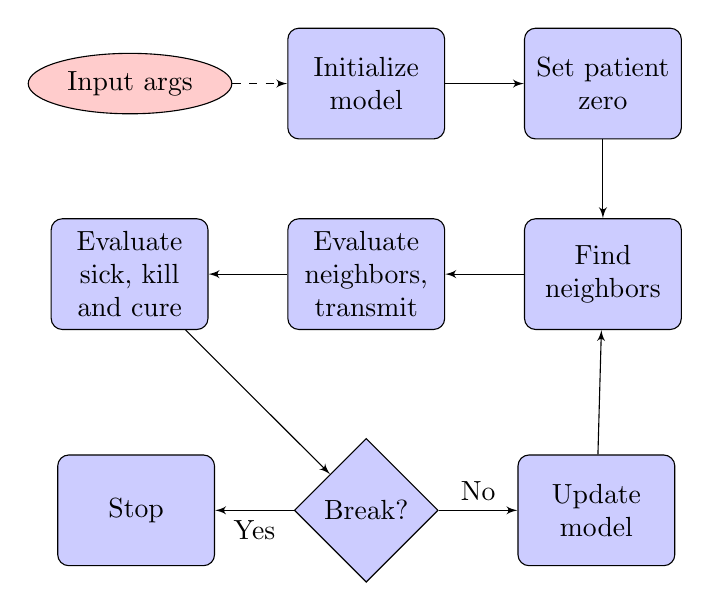
\begin{tikzpicture}[node distance = 1cm, auto,scale=2]
        % Place nodes
        \node [block] (init) {Initialize model};
        \node [cloud, left of=init] (expert) {Input args};
        \node [block, right= of init] (identify) {Set patient zero};
        \node [block, below= of identify] (evaluate) {Find neighbors};
        \node [block, left= of evaluate] (transmit) {Evaluate neighbors, transmit};
        \node [block, left= of transmit] (cure) {Evaluate sick, kill and cure};
        \node [decision, below of = transmit] (decide) {Break?};
        \node [block, right= of decide, node distance=3cm] (update) {Update model};
        \node [block, left= of decide, node distance=3cm] (stop) {Stop};
        % Draw edges
        \path [line,dashed] (expert) -- (init);
        \path [line] (init) -- (identify);
        \path [line] (identify) -- (evaluate);
        \path [line] (evaluate) -- (transmit);
        \path [line] (transmit) -- (cure);
        \path [line] (decide) -- node {No} (update);
        \path [line] (update) -- (evaluate);
        \path [line] (decide) -- node {Yes} (stop);
        \path [line] (cure) -- (decide);
    \end{tikzpicture}
\end{figure}

}

\section{Networks}
\frame{
\frametitle{Networks}

\begin{itemize}[label=\textbullet]
    \item Small world
    \item Scale free
    \item Random
    \item Custom network (two cities with commuters. Random networks for each city)
\end{itemize}

}

\section{Networks}
\frame{
\frametitle{Movie time: two cities, death}

\centering
\href{run:test.m4v}{Movie time: two cities, death}

}

\section{Networks}
\frame{
\frametitle{Movie time: two cities, immunity}

\centering
\href{run:./immune1.m4v}{Movie time: two cities, immunity}

}

\section{Custom network}
\frame{
\frametitle{Custom network}

\begin{figure}[ht]
\begin{tikzpicture}
    \begin{axis} [
        xticklabels={,,},
        yticklabels={,,},
        title={Custom network, simulating two cities with commuters},
        hide axis
        ]
        \addplot graphics [xmin=0,xmax=10,ymin=0,ymax=1] {../mads/test.png};
    \end{axis}
\end{tikzpicture}
\label{fig:network_twotowns}
\end{figure}

}

\section{Success criteria}
\frame{
\frametitle{Success criteria}

\begin{itemize}[label=\textbullet]
    \item Real world
    \begin{itemize}[label=\textbullet]
        \item Disease no longer endemic
    \end{itemize}
    \item Our model
    \begin{itemize}[label=\textbullet]
        \item Discussion of alternate criteria
        \begin{itemize}[label=\textbullet]
        	\item Percolation
        	\pause
            \item \textbf{Total sick \( < \) arbitrary threshold}
            \pause
            \item Effective reproductive number \( \leq 1 \)
            \pause
            \item \( n_{\text{sick}} = 0 \) and \( n_{\text{healthy}} \neq 0 \)
            \pause
            \item \( n_{\text{healthy}} = 0 \)
        \end{itemize}
    \end{itemize}
\end{itemize}

}

\section{The simulations}
\frame{
\frametitle{The simulations}

\begin{itemize}[label=\textbullet]
    \item Test 20 values of \(p_I\) (0 to 0.95, in steps of 0.05)
    \pause
    \item For each \(p_I\) test 50 different networks, and test each network 50 times (random distribution of patient zero and immune nodes)
    \pause
    \item Save relevant output
\end{itemize}

}

\section{Results}
\frame{
\frametitle{Results}

\begin{figure}
    \centering
    \begin{tikzpicture}
        \begin{axis}[
            legend pos=outer north east,
            xlabel=Fraction immune,
            ylabel=Fraction of runs with no. of sick \( \leq 5 \),
            title={Ebola, \( N = 1000, R_0=2 \)},
            %mlineplot,
            xmin=0,
            ymin=0.4,
            cycle list = color,
            y tick label style={
                    /pgf/number format/.cd,
                    fixed,
                    fixed zerofill,
                    precision=2,
                    /tikz/.cd
                }
            ]
            \addplot [only marks,red] table [col sep=comma,x index = {0}, y index = {1}, y error index = {2}] {../nikolai/csv/Ebola_smallworld.csv};
            \addlegendentry{Small world}
            \addplot [only marks,blue] table [col sep=comma,x index = {0}, y index = {1}, y error index = {2}] {../nikolai/csv/Ebola_scalefree.csv};
            \addlegendentry{Scale free}
            \addplot [only marks] table [col sep=comma,x index = {0}, y index = {1}, y error index = {2}] {../nikolai/csv/Ebola_random.csv};
            \addlegendentry{Random}
            \draw [dashed,red] (0.33,0) -- (0.33,1.3);
            \draw [dashed,red] (0.6,0) -- (0.6,1.3);
        \end{axis}
    \end{tikzpicture}
\end{figure}

}

\frame{
\frametitle{Results}

\begin{figure}
    \centering
    \begin{tikzpicture}
        \begin{axis}[
            legend pos=outer north east,
            xlabel=Fraction immune,
            ylabel=Fraction of runs with no. of sick \( \leq 5 \),
            title={Polio, \( N = 1000, R_0=6 \)},
            %mlineplot,
            cycle list=mlineplot cycle,
            xmin=0,
            ymin=0.4,
            y tick label style={
                    /pgf/number format/.cd,
                    fixed,
                    fixed zerofill,
                    precision=2,
                    /tikz/.cd
                }
            ]
            \addplot [only marks,red] table [col sep=comma,x index = {0}, y index = {1}, y error index = {2}] {../nikolai/csv/Polio_smallworld.csv};
            \addlegendentry{Small world}
            \addplot [only marks,blue] table [col sep=comma,x index = {0}, y index = {1}, y error index = {2}] {../nikolai/csv/Polio_scalefree.csv};
            \addlegendentry{Scale free}
            \addplot [only marks] table [col sep=comma,x index = {0}, y index = {1}, y error index = {2}] {../nikolai/csv/Polio_random.csv};
            \addlegendentry{Random}
            \draw [dashed,red] (0.8,0) -- (0.8,1.3);
            \draw [dashed,red] (0.86,0) -- (0.86,1.3);
        \end{axis}
    \end{tikzpicture}
\end{figure}

}

\frame{
\frametitle{Results}

\begin{figure}
    \centering
    \begin{tikzpicture}
        \begin{axis}[
            legend pos=outer north east,
            xlabel=Fraction immune,
            ylabel=Fraction of runs with no. of sick \( \leq 5 \),
            title={Measles, \( N = 1000, R_0=15 \)},
            %mlineplot,
            cycle list=mlineplot cycle,
            xmin=0,
            ymin=0.4,
            y tick label style={
                    /pgf/number format/.cd,
                    fixed,
                    fixed zerofill,
                    precision=2,
                    /tikz/.cd
                }
            ]
            \addplot [only marks,red] table [col sep=comma,x index = {0}, y index = {1}, y error index = {2}] {../nikolai/csv/Measles_smallworld.csv};
            \addlegendentry{Small world}
            \addplot [only marks,blue] table [col sep=comma,x index = {0}, y index = {1}, y error index = {2}] {../nikolai/csv/Measles_scalefree.csv};
            \addlegendentry{Scale free}
            \addplot [only marks] table [col sep=comma,x index = {0}, y index = {1}, y error index = {2}] {../nikolai/csv/Measles_random.csv};
            \addlegendentry{Random}
            \draw [dashed,red] (0.92,0) -- (0.92,1.3);
            \draw [dashed,red] (0.94,0) -- (0.94,1.3);
        \end{axis}
    \end{tikzpicture}
\end{figure}

}



\section{Conclusion}
\frame{
\frametitle{Conclusion}

\begin{itemize}
    \item Simulating the spread of disease is easy. Defining herd immunity is hard.
\end{itemize}


}

\end{document}
